\begin{textbox}{\href{https://compneuro.neuromatch.io/tutorials/W3D3_OptimalControl/student/W3D3_Tutorial1.html}{Optimal Control for Discrete States }   }
\begin{subbox}{subbox}{Overview}
\scriptsize
Optimal Control combines ideas from the Hidden Dynamics lessons (which used Hidden Markov Models) with maximizing utility described in the Bayes day (which combined a posterior with a utility function). It also connects directly to later lessons in Reinforcement Learning, which learns how to control before you understand the world. In contrast, Optimal Control assumes that you already know how the world works.

Optimal Control is a crucial model in motor neuroscience, because it provides a principled benchmark for how we expect an animal should move. It also is an important engineering method, used for brain-computer interfaces and clamping neurons to desired activity patterns.

\end{subbox}

\begin{subbox}{subbox}{Objective}
\scriptsize
Here, we will implement a \textbf{binary control} task: a Partially Observable Markov Decision Process (POMDP) that describes fishing. The agent (you) seeks reward from two fishing sites without directly observing where the school of fish is (yes, a group of fish is called a school!). This makes the world a Hidden Markov Model (HMM). Based on when and where you catch fish, you keep updating your belief about the fish location, i.e., the posterior of the fish given past observations. You should control your position to get the most fish while minimizing the cost of switching sides.

You've already learned about stochastic dynamics, latent states, and measurements. These first exercises largely repeat your previous work. Now we introduce \textbf{actions}, based on the new concepts of \textbf{control, utility, and policy}. This general structure provides a foundational model for the brain's computations because it includes a perception-action loop where the animal can gather information, draw inferences about its environment, and select actions with the greatest benefit. \textit{How}, mechanistically, the neurons could actually implement these calculations is a separate question we don't address in this lesson.

We will:
\begin{itemize}
    \item 
 Use the Hidden Markov Models you learned about previously to model the world state.
    \item  Use the observations (fish caught) to build beliefs (posterior distributions) about the fish location.
    \item  Evaluate the quality of different control policies for choosing actions.
    \item  Discover the policy that maximizes utility.
\end{itemize}

\end{subbox}
\end{textbox}
%%%%%%%%%%%%%%%%%%%%%%%%% 
%%%%%%%%%%%%%%%%%%%%%%%%%
\begin{textbox}{\href{https://compneuro.neuromatch.io/tutorials/W3D3_OptimalControl/student/W3D3_Tutorial1.html}{Optimal Control for Discrete States }   }
\begin{subbox}{subbox}{Analyzing the Problem}
\scriptsize
\textbf{Problem Setting}\\

\textbf{1. State dynamics:} There are two possible locations for the fish: Left and Right. Secretly, at each time step, the fish may switch sides with a certain probability $p_{\rm sw} = 1 - p_{\rm stay}$. This is the binary switching model (\textit{Telegraph process}) that you've seen in Linear Systems . The fish location, $s^{\rm fish}$, is latent; you get measurements about it when you try to catch fish, like in Hidden Dynamics. This gives you a \textit{belief} or posterior probability of the current location given your history of measurements.\\

\textbf{2. Actions}: Unlike past days, you can now \textbf{act} on the process! You may stay on your current location (Left or Right), or switch to the other side.\\

\textbf{3. Rewards and Costs:} You get rewarded for each fish you catch (one fish is worth 1 "point"). If you're on the same side as the fish, you'll catch more, with probability $q_{\rm high}$ per discrete time step. Otherwise, you may still catch some fish with probability $q_{\rm low}$. \\

You pay a price of $C$ points for switching to the other side. So you better decide wisely!

\textbf{Maximizing Utility}\\

To decide "wisely" and maximize your total utility (total points), you will follow a \textbf{policy} that prescribes what to do in any situation. Here the situation is determined by your location and your \textbf{belief} $b_t$ (posterior) about the fish location (remember that the fish location is a latent variable). 

In optimal control theory, the belief is the posterior probability over the latent variable given all the past measurements. It can be shown that maximizing the expected utility with respect to this posterior is optimal.

In our problem, the belief can be represented by a single number because the fish are either on the left or the right side. So we write: 

\begin{equation}
b_t = p(s^{\rm fish}_t = {\rm Right}\  |\  m_{0:t}, a_{0:t-1})
\end{equation}

where $m_{0:t}$ are the measurements and $a_{0:t-1}$ are the actions (stay or switch).

Finally, we will parameterize the policy by a simple threshold on beliefs: when your belief that fish are on your current side falls below a threshold $\theta$, you switch to the other side.

Here, you will discover that if you pick the right threshold, this simple policy happens to be optimal!

\end{subbox}

\end{textbox}
%%%%%%%%%%%%%%%%%%%%%%%%% 
%%%%%%%%%%%%%%%%%%%%%%%%%
\begin{textbox}{\href{https://compneuro.neuromatch.io/tutorials/W3D3_OptimalControl/student/W3D3_Tutorial1.html}{Optimal Control for Discrete States }   }
\begin{subbox}{subbox}{Analyzing the Problem}
\scriptsize
\textbf{Problem Setting}\\

\textbf{1. State dynamics:} There are two possible locations for the fish: Left and Right. Secretly, at each time step, the fish may switch sides with a certain probability $p_{\rm sw} = 1 - p_{\rm stay}$. This is the binary switching model (\textit{Telegraph process}) that you've seen in Linear Systems . The fish location, $s^{\rm fish}$, is latent; you get measurements about it when you try to catch fish, like in Hidden Dynamics. This gives you a \textit{belief} or posterior probability of the current location given your history of measurements.\\

\textbf{2. Actions}: Unlike past days, you can now \textbf{act} on the process! You may stay on your current location (Left or Right), or switch to the other side.\\

\textbf{3. Rewards and Costs:} You get rewarded for each fish you catch (one fish is worth 1 "point"). If you're on the same side as the fish, you'll catch more, with probability $q_{\rm high}$ per discrete time step. Otherwise, you may still catch some fish with probability $q_{\rm low}$. \\

You pay a price of $C$ points for switching to the other side. So you better decide wisely!

\textbf{Maximizing Utility}\\

To decide "wisely" and maximize your total utility (total points), you will follow a \textbf{policy} that prescribes what to do in any situation. Here the situation is determined by your location and your \textbf{belief} $b_t$ (posterior) about the fish location (remember that the fish location is a latent variable). 

In optimal control theory, the belief is the posterior probability over the latent variable given all the past measurements. It can be shown that maximizing the expected utility with respect to this posterior is optimal.

In our problem, the belief can be represented by a single number because the fish are either on the left or the right side. So we write: 

\begin{equation}
b_t = p(s^{\rm fish}_t = {\rm Right}\  |\  m_{0:t}, a_{0:t-1})
\end{equation}

where $m_{0:t}$ are the measurements and $a_{0:t-1}$ are the actions (stay or switch).

Finally, we will parameterize the policy by a simple threshold on beliefs: when your belief that fish are on your current side falls below a threshold $\theta$, you switch to the other side.

Here, you will discover that if you pick the right threshold, this simple policy happens to be optimal!

\end{subbox}

\end{textbox}
%%%%%%%%%%%%%%%%%%%%%%%%% 
%%%%%%%%%%%%%%%%%%%%%%%%%
\begin{textbox}{\href{https://compneuro.neuromatch.io/tutorials/W3D3_OptimalControl/student/W3D3_Tutorial1.html}{Optimal Control for Discrete States }   }


\begin{subbox}{subbox}{ Examining fish dynamics}
\scriptsize

Look at the dynamics of the fish moving from side to side while you stay in one place. With the probability (stay prob=0.9) of fish staying in the same location, and observe the resulting dynamics of the fish.

\begin{center}
    
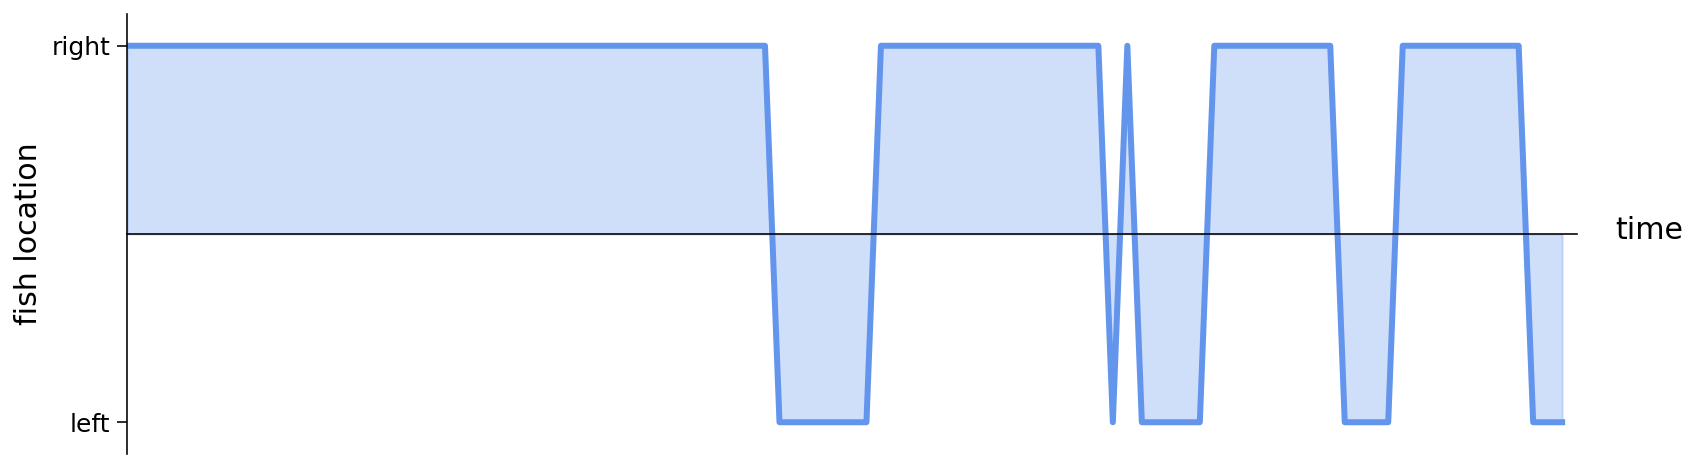
\includegraphics[scale=0.2]{Figures/OC/OC_Figure1.png}
\end{center}

\end{subbox}
\begin{subbox}{subbox}{ Examining the reward function}
\scriptsize

You can control your location, but we fix the fish's location by setting `stay prob = 1`. Now that the fish are serenely swimming in one location, we can visually inspect the rewards when you're on the same side as the fish or on the other side.

When you're on the same side as the fish, you should have a higher probability of catching them (but watch out, since technically, you are \textit{allowed} to adjust the sliders to other conditions!).

\begin{center}
    
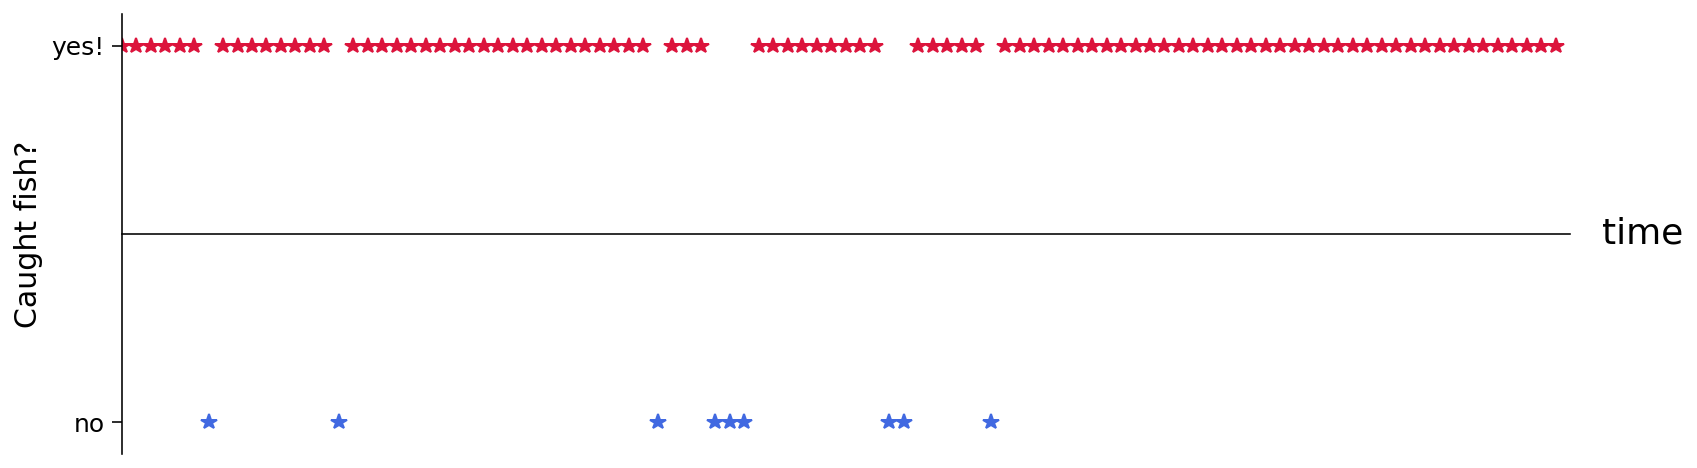
\includegraphics[scale=0.2]{Figures/OC/OC_Figure2.png}
\end{center}

\end{subbox}
\begin{subbox}{subbox}{ Belief dynamics and belief distributions}
\scriptsize

Now it's time to get an intuition on how beliefs are calculated. Here we define your belief about the fish location is just the posterior probability about that location given your measurements, $p(s_t|m_{0:t})$. Note that this is just like Hidden Dynamics!

If you'll always stay on the LEFT side, but the fish will move around. They'll stay on the same side with probability `stay prob`. You only get to see fish you catch, not where the school of fish is. You have to use those measurements to infer the location of the school.

\begin{center}
    
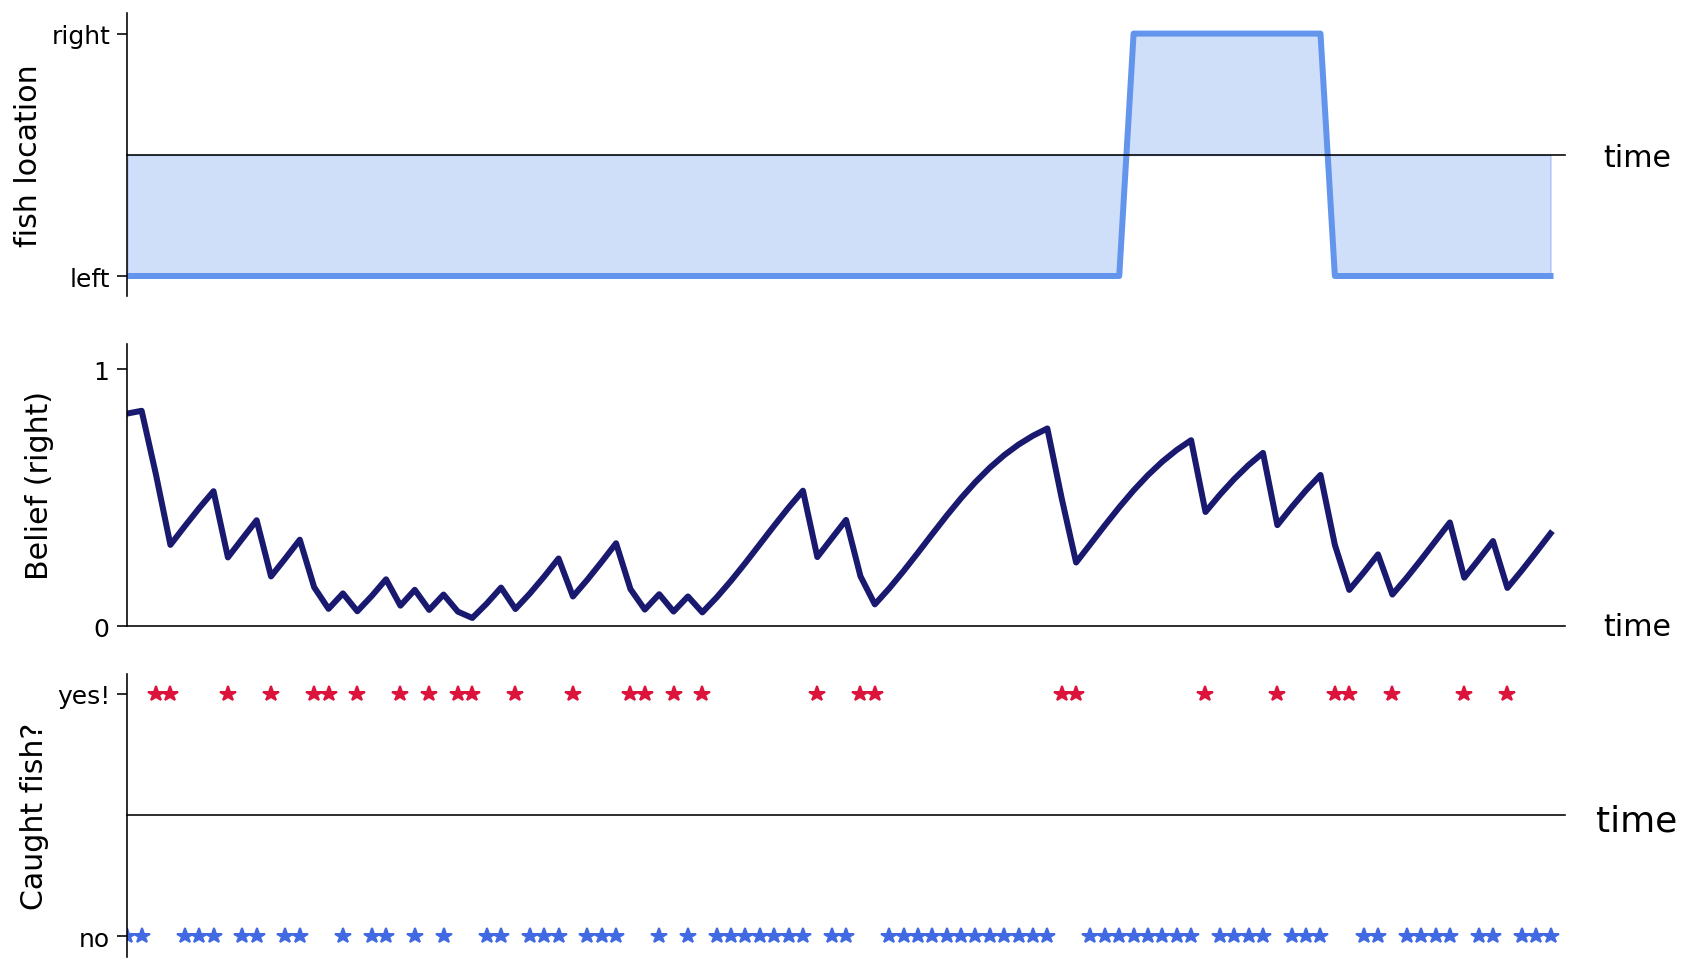
\includegraphics[scale=0.21]{Figures/OC/OC_Figure3.png}
\end{center}

\end{subbox}
\end{textbox}
%%%%%%%%%%%%%%%%%%%%%%%%% 
%%%%%%%%%%%%%%%%%%%%%%%%%
\begin{textbox}{\href{https://compneuro.neuromatch.io/tutorials/W3D3_OptimalControl/student/W3D3_Tutorial1.html}{Optimal Control for Discrete States }   }


\begin{subbox}{subbox}{ Implementing a threshold policy}
\scriptsize

Now we'll switch the policy from the lazy policy used above to a threshold policy. You'll change your location whenever your belief is low enough that you're on the best side. This policy takes three inputs: 
\begin{enumerate}
    \item 
 The \textit{belief} about the fish state. For convenience, we will represent the belief at time $t$ using a 2-dimensional vector. The first element is the belief that the fish are on the left, and the second element is the belief the fish are on the right. At every time step, these elements sum to 1.

\item  Your location, represented as "Left" = -1 and "Right" = 1. 

\item  A belief \textit{threshold} that determines when to switch. When your belief that you are on the same side as the fish drops below this threshold, you should move to the other location, and otherwise stay.
\end{enumerate}
\end{subbox}

\begin{subbox}{subbox}{ Dynamics with different thresholds}
\begin{center}
    
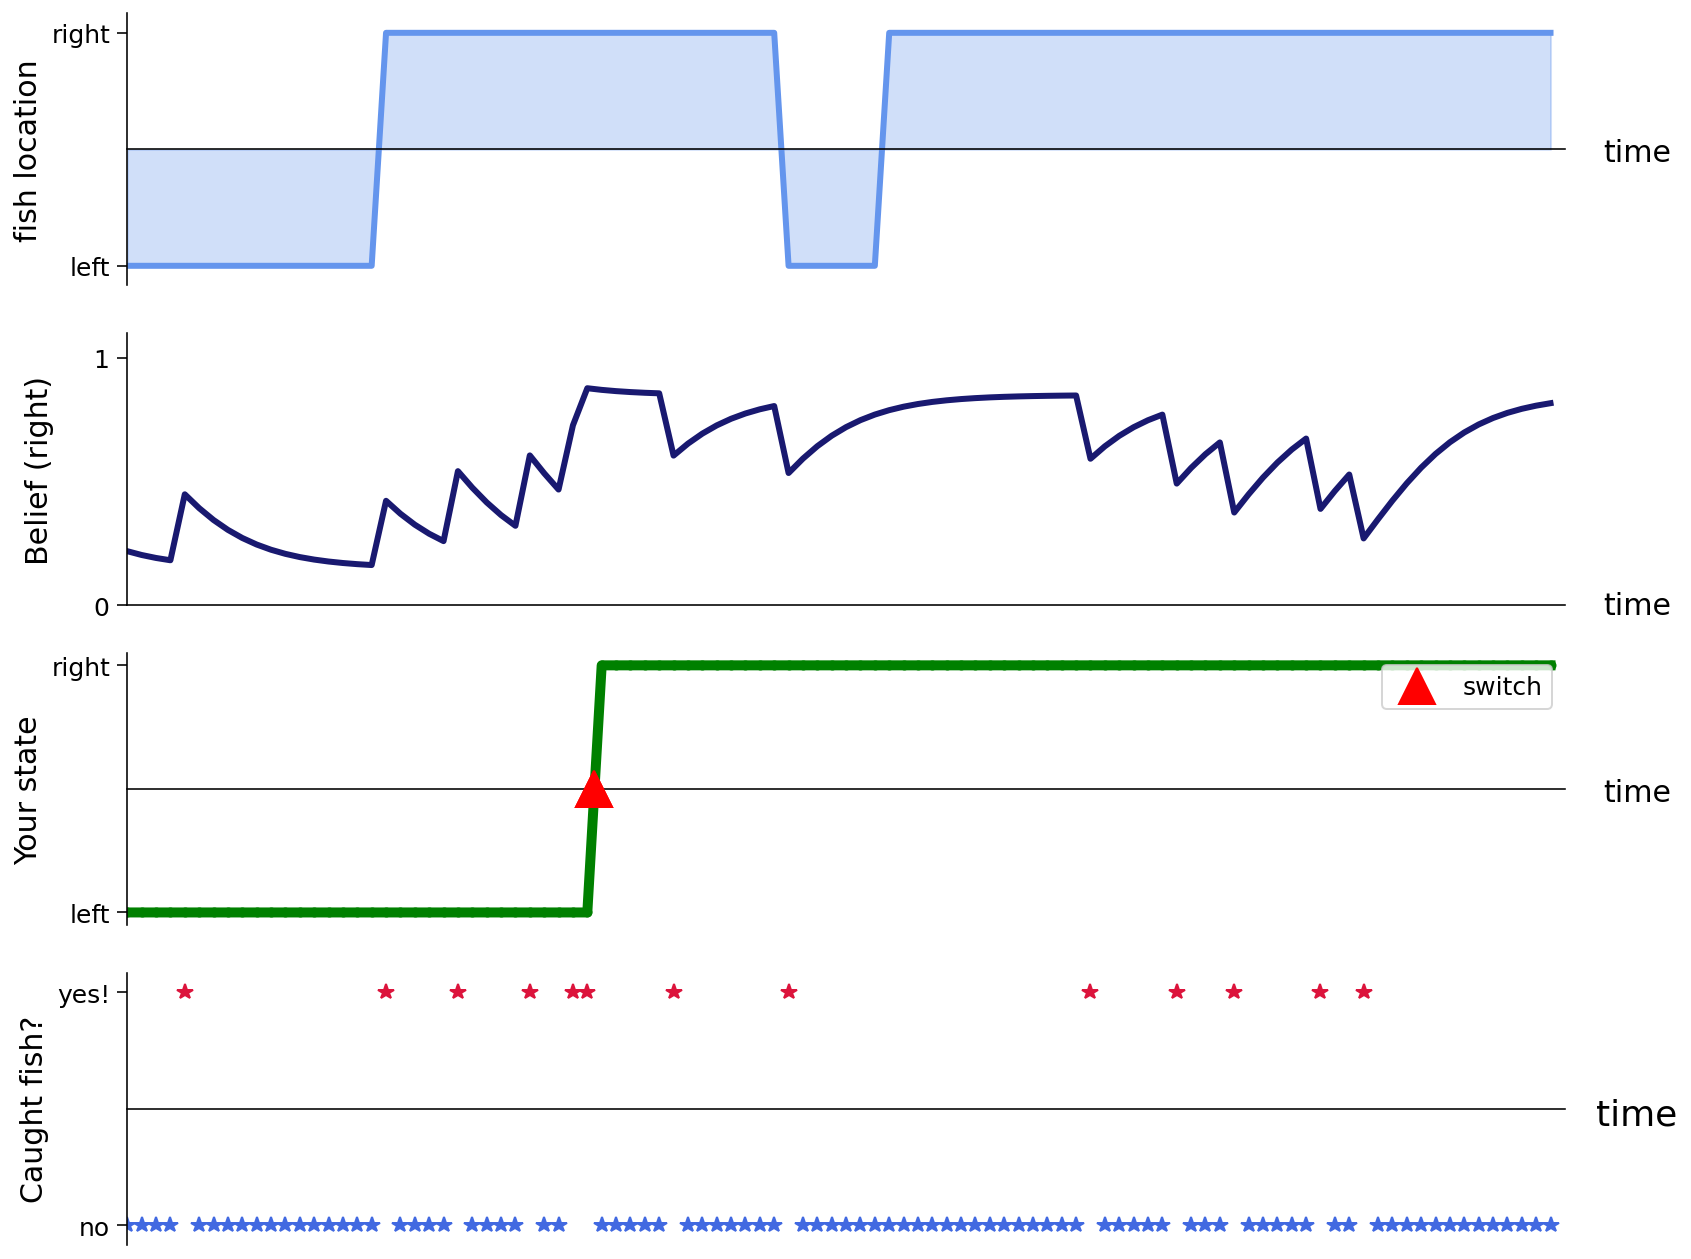
\includegraphics[scale=0.2]{Figures/OC/OC_Figure4.png}
\end{center}

\end{subbox}
\end{textbox}
%%%%%%%%%%%%%%%%%%%%%%%%% 
%%%%%%%%%%%%%%%%%%%%%%%%%
\begin{textbox}{\href{https://compneuro.neuromatch.io/tutorials/W3D3_OptimalControl/student/W3D3_Tutorial1.html}{Optimal Control for Discrete States }   }
\begin{subbox}{subbox}{ Implementing a value function}
\scriptsize

Let's find out how good our threshold is. For that, we will calculate a \textbf{value function} that quantifies our utility (total points). We will use this value to compare different thresholds; remember, our goal is to maximize the amount of fish we catch while minimizing the effort involved in changing locations.

The value is the total expected utility per unit time.

\begin{equation}
V(\theta) = \frac{1}{T}\left( \sum_t R(s_t) - C(a_t) \right)
\end{equation}

where $R(s_t)$ is the instantaneous reward we get at location $s_t$ and $C(a_t)$ is the cost we paid for the chosen action. Remember, we receive one point for fish caught and pay cost points for switching to the other location. 

We could take this average mathematically over the probabilities of rewards and actions. However, we can get the same answer by simply averaging the \textit{actual} rewards and costs over a long time.


\begin{center}
    
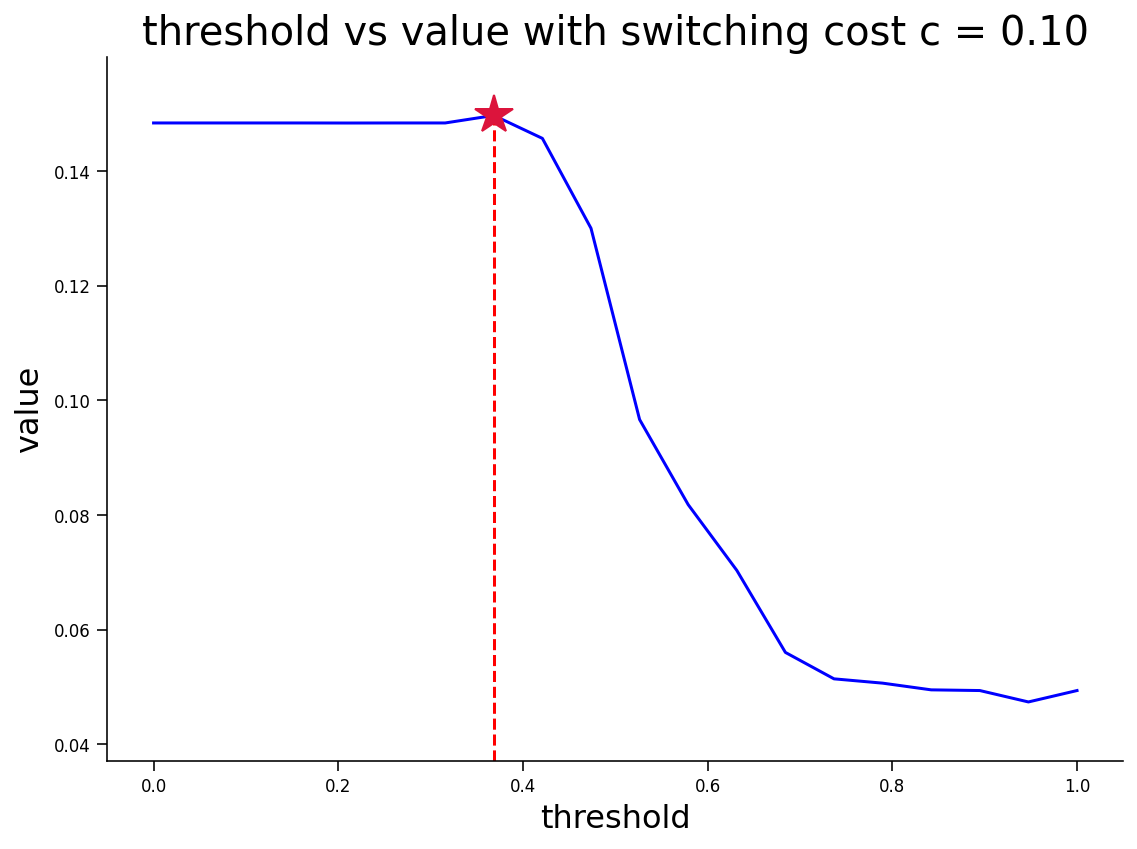
\includegraphics[scale=0.15]{Figures/OC/OC_Figure5.png}
\end{center}

\end{subbox}

\begin{subbox}{subbox}{ Summary}
\scriptsize
In this tutorial, you combined Hidden Markov Models with actions to solve an optimal control problem! This showed us the core formalism of the \textit{Partially Observable Markov Decision Process} (POMDP).

Using observations (fish caught), you built beliefs (posterior distributions) that helped you estimate where the fish were. Next, you computed a value function that helped you evaluate the quality of different policies. Finally, using a brute force approach, you discovered an optimal policy that allowed you to catch as many fish as possible while minimizing the effort of switching your location.

The following tutorial will use continuous states and actions instead of the binary ones we used here. In continuous control, we can still use a POMDP, but we'll focus on control in the fully observed case, a Markov Decision Process (MDP), since the policy is still illuminating.

\end{subbox}
\end{textbox}
%%%%%%%%%%%%%%%%%%%%%%%%% 
%%%%%%%%%%%%%%%%%%%%%%%%%
\begin{textbox}{\href{https://compneuro.neuromatch.io/tutorials/W3D3_OptimalControl/student/W3D3_Tutorial2.html}{Optimal Control for Continuous State}}
\begin{subbox}{subbox}{ Exploring a Linear Dynamical System (LDS) with Open-Loop and Closed-Loop Control}
\scriptsize


In this example, a cat is trying to catch a mouse in space. The location of the mouse is the goal state $g$, here a static goal. Later on, we will make the goal time-varying, i.e., $g(t)$. The cat's location is the state of the system $s_t$. The state has its internal dynamics: think of the cat drifting slowly in space. These dynamics are such that the state at the next time step $s_{t+1}$ are a linear function of the current state $s_t$. There is some process noise affecting the state (think about engine corrosions on the little jetpack causing unintended movements) here modeled as Gaussian noise $w_t$.

The control input or action $a_t$ is the action of the jet pack, which has an effect $Ba_t$ on the state at the next time step $s_{t+1}$. Here, we will be designing the action $a_t$ to reach the goal $g$, with known state dynamics.

Thus, our linear discrete-time system evolves according to the following equation:
\begin{eqnarray*}
s_{t+1} &=& Ds_t + Ba_t + w_t \tag{1}\\
s_{0} &=& s_{init}
\end{eqnarray*}
with,\\
$t$: time step, ranging from $1$ to $T$, where $T$ is the time horizon.\\
$s_t$: state at time $t$.\\
$a_t$: action at time $t$ (also known as "control input").\\
$w_t$: gaussian noise at time $t$.\\
$D$: transition matrix.\\
$B$: input matrix.\\

For simplicity, we will consider the 1D case, where the matrices reduce to scalars, and the states, control and noise are one-dimensional as well. Specifically, $D$ and $B$ are scalars.

We will consider the goal $g$ to be the origin, i.e., $g=0$, for Exercises 1 and 2.2. Later on, we will explore scenarios where the goal state changes over time $g(t)$.\\



\textbf{Stability}\\

The system is stable, i.e., the output remains finite for any finite initial condition $s_{init}$, if $|D| < 1$. Note that if the state dynamics are stable, the state eventually reaches $0$ (No control is needed!). However, when $|D|>1$ or the goal $g \neq 0$ selecting an appropriate sequence of actions becomes essential to completing the task.\\


\textbf{Open-loop control and Closed-loop linear control}\\

In \textit{open-loop control}, $a_t$ is not a function of $s_t$. In *closed-loop linear control*, $a_t$ is a linear function of the state $s_t$. Specifically, $a_t$ is the control gain, $L_t$, multiplied by $s_t$, i.e., $a_t=L_t s_t$. 


\end{subbox}
\end{textbox}
%%%%%%%%%%%%%%%%%%%%%%%%% 
%%%%%%%%%%%%%%%%%%%%%%%%%
\begin{textbox}{\href{https://compneuro.neuromatch.io/tutorials/W3D3_OptimalControl/student/W3D3_Tutorial2.html}{Optimal Control for Continuous State}}
\begin{subbox}{subbox}{ Explore no control vs. open-loop control vs. closed-loop control}
\scriptsize

The plot below visualizes the effects of different kinds of control inputs.\\
1.  For the no-control case, can you identify two distinct outcomes, depending on the value of D? Why?\\
2.  The open-loop controller works well--or does it? Are there any problems in in challenging (high noise) conditions.\\
3. Does the closed-loop controller fare better with the noise? Vary the values of $L$ and find a range where it quickly reaches the goal.

\begin{center}
    
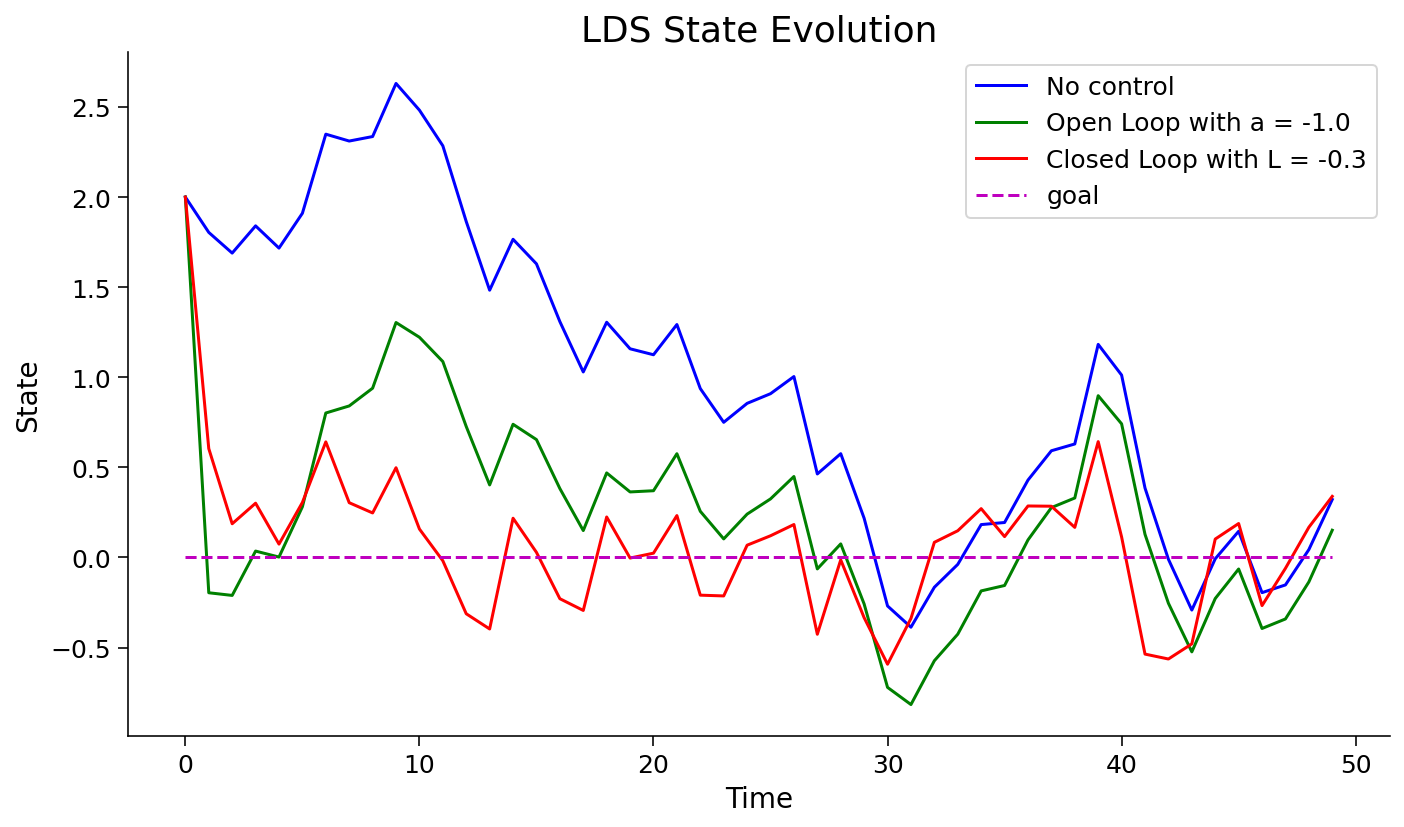
\includegraphics[scale=0.2]{Figures/OC/OC_Figure6.png}
\end{center}

\end{subbox}

\begin{subbox}{subbox}{ Exploring the closed-loop setting further }
\scriptsize

The plot below visualizes the MSE between the state and goal, as a function of control gain $L$. You should see a U-shaped curve, with a minimum MSE. The control gain at which the minimum MSE is reached, is the optimal constant control gain for minimizing MSE, here called the numerical optimum. 

A green dashed line is shown $L = -\frac{D}{B}$ with $D=1.1$ and $B=2$. Why is this the theoretical optimal control gain for minimizing MSE of the state $s$ to the goal $g=0$? Examine how the states evolve with a constant gain $L$.
\begin{eqnarray*}
s_{t+1} &=& Ds_t + Ba_t + w_t \\
&=& Ds_t + B(Ls_t) + w_t \\
&=& (D+BL)s_t + w_t \tag{2}
\end{eqnarray*}

\begin{center}
    
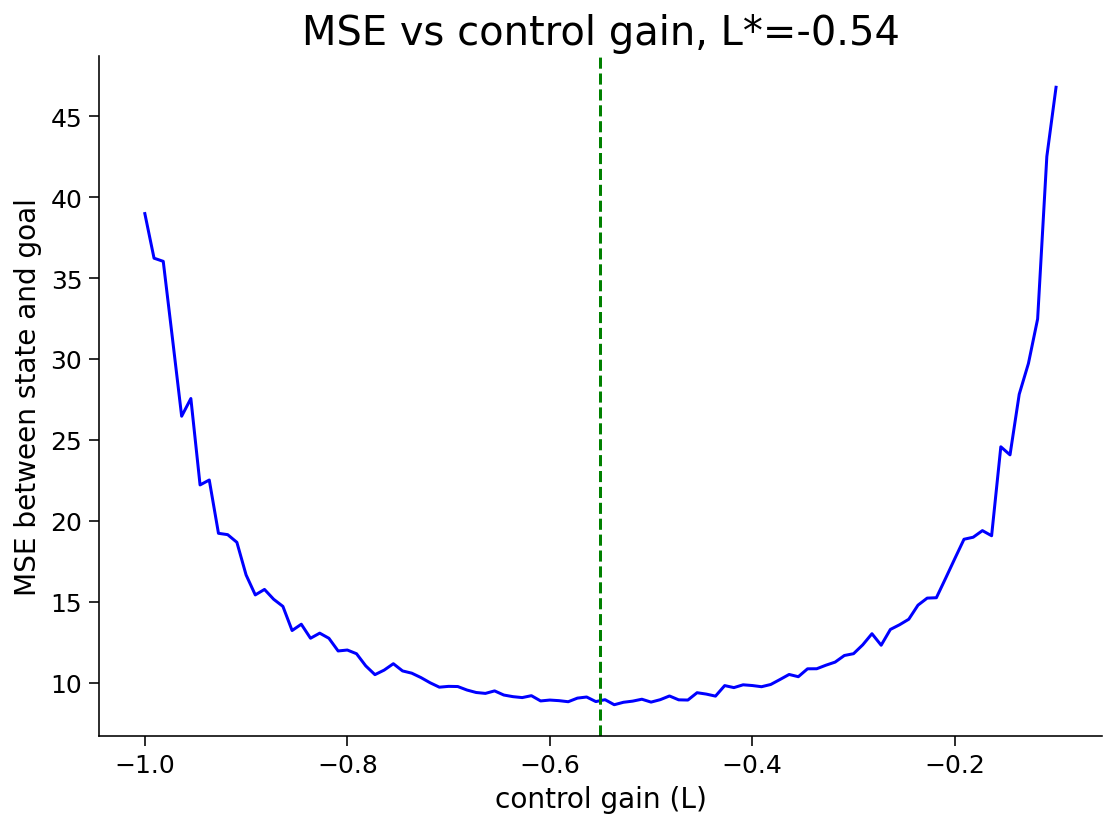
\includegraphics[scale=0.2]{Figures/OC/OC_Figure7.png}
\end{center}

\end{subbox}
\end{textbox}
%%%%%%%%%%%%%%%%%%%%%%%%% 
%%%%%%%%%%%%%%%%%%%%%%%%%
\begin{textbox}{\href{https://compneuro.neuromatch.io/tutorials/W3D3_OptimalControl/student/W3D3_Tutorial2.html}{Optimal Control for Continuous State}}
\begin{subbox}{subbox}{ Explore no control vs. open-loop control vs. closed-loop control}
\scriptsize
Now, let's visualize the evolution of the system as we change the control gain. 

\begin{center}
    
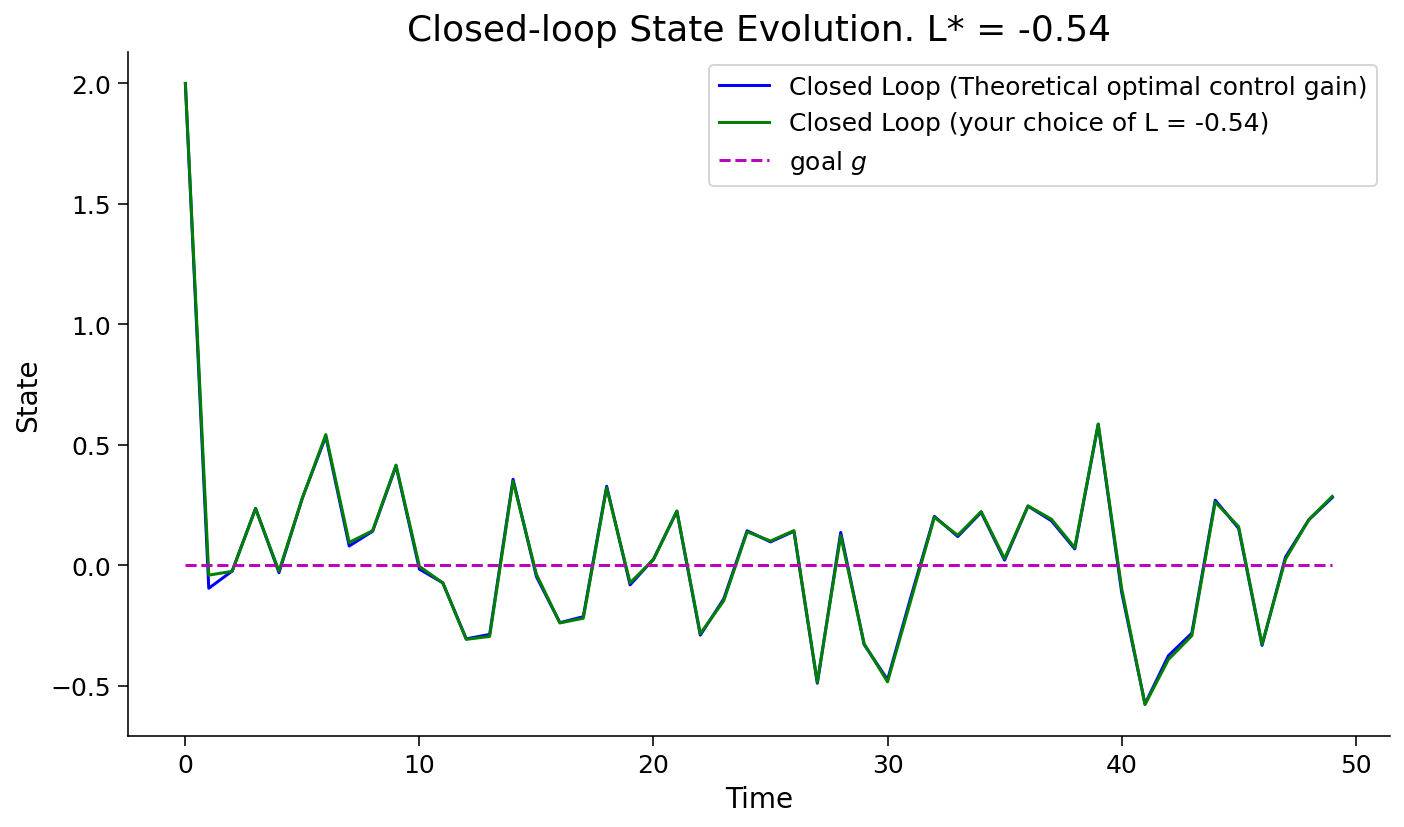
\includegraphics[scale=0.2]{Figures/OC/OC_Figure8.png}
\end{center}


\end{subbox}

\begin{subbox}{subbox}{ Designing an optimal control input using a linear quadratic regulator (LQR)}
\scriptsize
\textbf{Constraints on the system}\\
Now we will start imposing additional constraints on our system. For example, if you explored different values for $s_{init}$ above, you would have seen very large values for $a_t$ in order to get to the mouse in a short amount of time. However, perhaps the design of our jetpack makes it dangerous to use large amounts of fuel in a single timestep. We certainly do not want to explode, so we would like to keep the actions $a_t$ as small as possible while still maintaining good control.

Moreover, we had restricted ourselves to a static control gain $L_t \equiv L$. How would we vary it if we could?

This leads us to a more principled way of designing the optimal control input.

\textbf{Setting up a cost function}\\

In a finite-horizon LQR problem,  the cost function is defined as: 
\begin{eqnarray*}
J({\bf s},{\bf a}) &=& J_{state}({\bf s}) + \rho J_{control}({\bf a}) \\
 &=& \sum_{t = 0}^{T} (s_{t}-g)^2 + \rho \sum_{t=0}^{T-1}a_{t}^2 \tag{3}
\end{eqnarray*}
where $\rho$ is the weight on the control effort cost, as compared to the cost of not being at the goal. Here, ${\bf a} = \{a_t\}_{t=0}^{T-1}$, ${\bf s} = \{s_t\}_{t=0}^{T}$. This is a quadratic cost function. In Exercise $2$, we will only explore $g=0$, in which case $J_{state}({\bf s})$ can also be expressed as $\sum_{t = 0}^{T} s_{t}^2$. 


The goal of the LQR problem is to find control ${\bf a}$ such that $J({\bf s},{\bf a})$ is minimized. The goal is then to find the control gain at each time point, i.e.,

\begin{equation*}
\text{argmin} _{\{L_t\}_{t=0}^{T-1}}  J({\bf s},{\bf a}) 
\end{equation*}

where $a_t = L_t s_t$.


\end{subbox}


\end{textbox}
%%%%%%%%%%%%%%%%%%%%%%%%% 
%%%%%%%%%%%%%%%%%%%%%%%%%
\begin{textbox}{\href{https://compneuro.neuromatch.io/tutorials/W3D3_OptimalControl/student/W3D3_Tutorial2.html}{Optimal Control for Continuous State}}
\begin{subbox}{subbox}{ Designing an optimal control input using a linear quadratic regulator (LQR)}
\scriptsize

The solution to Equation for LQR for a finite time horizon, can be obtained via Dynamic Programming. For details, check out \href{https://stanford.edu/class/ee363/lectures/dlqr.pdf}{this lecture by Stephen Boyd}.\\
For an infinite time horizon, one can obtain a closed-form solution using Riccati equations, and the solution for the control gain becomes time-invariant, i.e., $L_t \equiv L$.  For  details, check out 
\href{https://stanford.edu/class/ee363/lectures/dlqr-ss.pdf}{this other lecture by Stephen Boyd}.\\
The cost function $J({\bf s}, {\bf a})$ can be divided into two parts: $J_{state}({\bf s})$ and $J_{control}({\bf a})$. 

\end{subbox}

\begin{subbox}{subbox}{ LQR to the origin }
\scriptsize

Here, we will use LQR controller to track a static goal at $g=0$. We will explore how varying $\rho$ (the weight on the control effort cost) affects the state trajectory, actions selected, and control gain.

\begin{center}
    
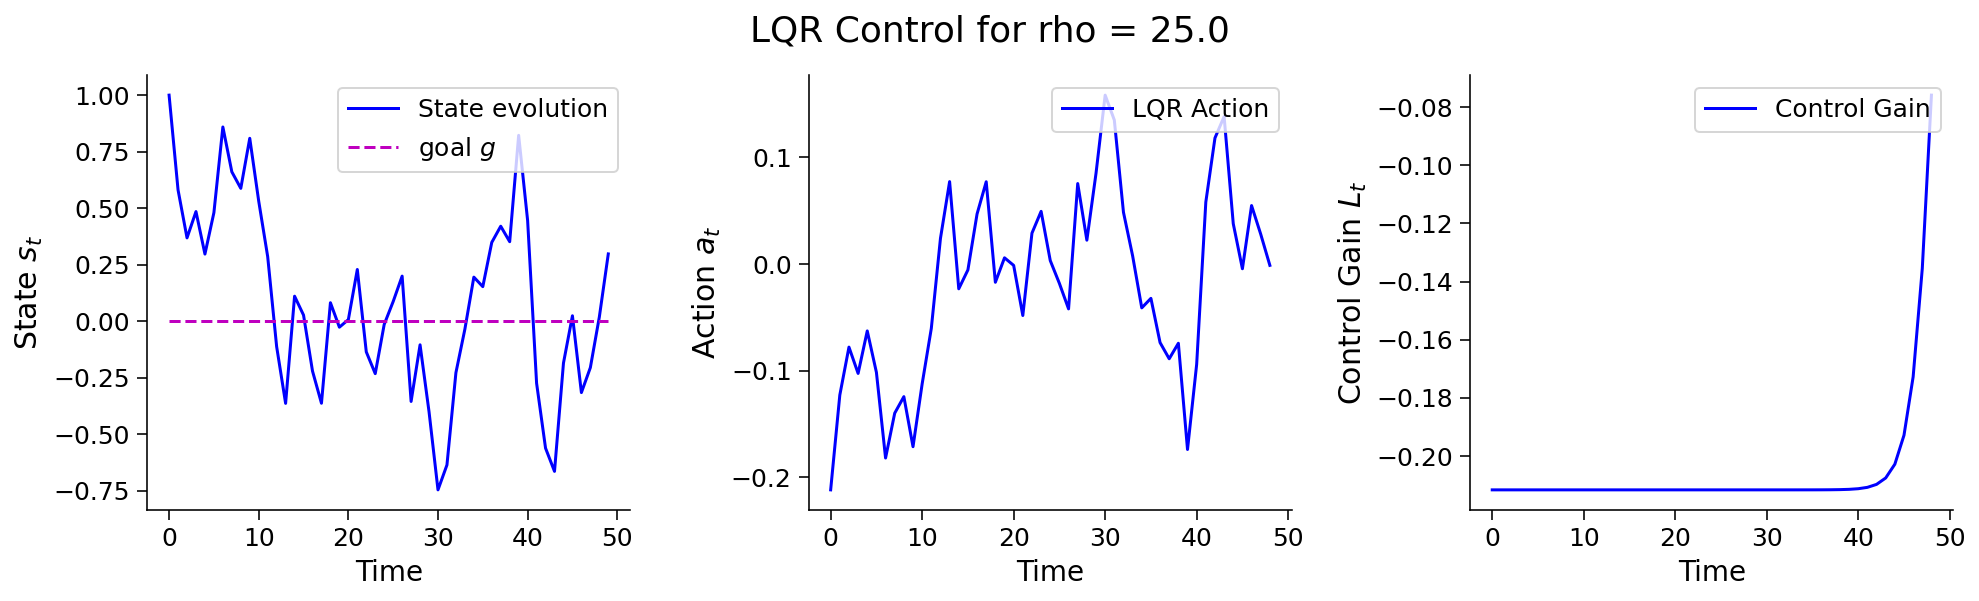
\includegraphics[scale=0.2]{Figures/OC/OC_Figure9.png}
\end{center}

\end{subbox}
\begin{subbox}{subbox}{ The tradeoff between state cost and control cost }
\scriptsize

We will now plot them against each other for varying values of $\rho$ to explore the tradeoff between state cost and control cost.
\begin{center}
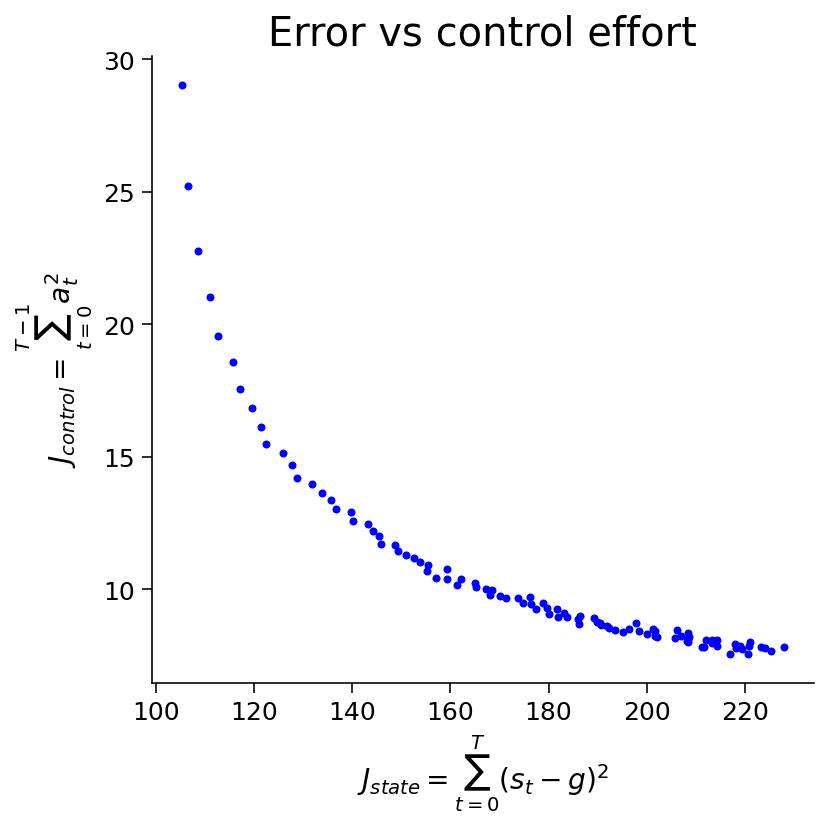
\includegraphics[scale=0.22]{Figures/OC/OC_Figure10.png}
\end{center}
You should notice the bottom half of the curve, forming the tradeoff between the state cost and the control cost under optimal closed-loop linear control.

For a desired value of the state cost, we cannot reach a lower control cost than the curve in the above plot. Similarly, for a desired value of the control cost, we must accept that amount of state cost. For example, if you know that you have a limited amount of fuel, which determines your maximum control cost to be $J_{control}^{max}$. 

You will be able to show that you will not be able to track your state with higher accuracy than the corresponding $J_{state}$ as given by the graph above. This is thus an important curve when designing a system and exploring its control.

\end{subbox}

\end{textbox}
%%%%%%%%%%%%%%%%%%%%%%%%% 
%%%%%%%%%%%%%%%%%%%%%%%%%
\begin{textbox}{\href{https://compneuro.neuromatch.io/tutorials/W3D3_OptimalControl/student/W3D3_Tutorial2.html}{Optimal Control for Continuous State}}


\begin{subbox}{subbox}{ LQR for tracking a time-varying goal}
\scriptsize

In a more realistic situation, the mouse would move around constantly. Suppose you were able to predict the movement of the mouse as it bounces from one place to another. This becomes your goal trajectory $g_t$.

When the target state, denoted as $g_t$, is not $0$, the cost function becomes

\begin{equation*}
J({\bf a}) = \sum_{t = 0}^{T} (s_{t}- g_t) ^2 + \rho \sum_{t=0}^{T-1}(a_{t}-\bar a_t)^2
\end{equation*}

Here, $\bar a_t$ is the desired action based on the goal trajectory. In other words, the controller considers the goal for the next time step, and designs a preliminary control action that gets the state at the next time step to the desired goal. Specifically, without taking into account noise $w_t$, we would like to design $\bar a_t$ such that $s_{t+1}=g_{t+1}$. Thus we have

\begin{eqnarray*}
g_{t+1} &=& Ds_t + B \bar a_t\\
\bar a_{t} &=& \frac{- Ds_t + g_{t+1}}{B}
\end{eqnarray*}

The final control action $a_t$ is produced by adding this desired action $\bar a_t$ with the term with the control gain $L_t(s_t - g_t)$.

The plot shows LQR tracks a time-varying goal for a  sinusoidal goal function.

\begin{center}
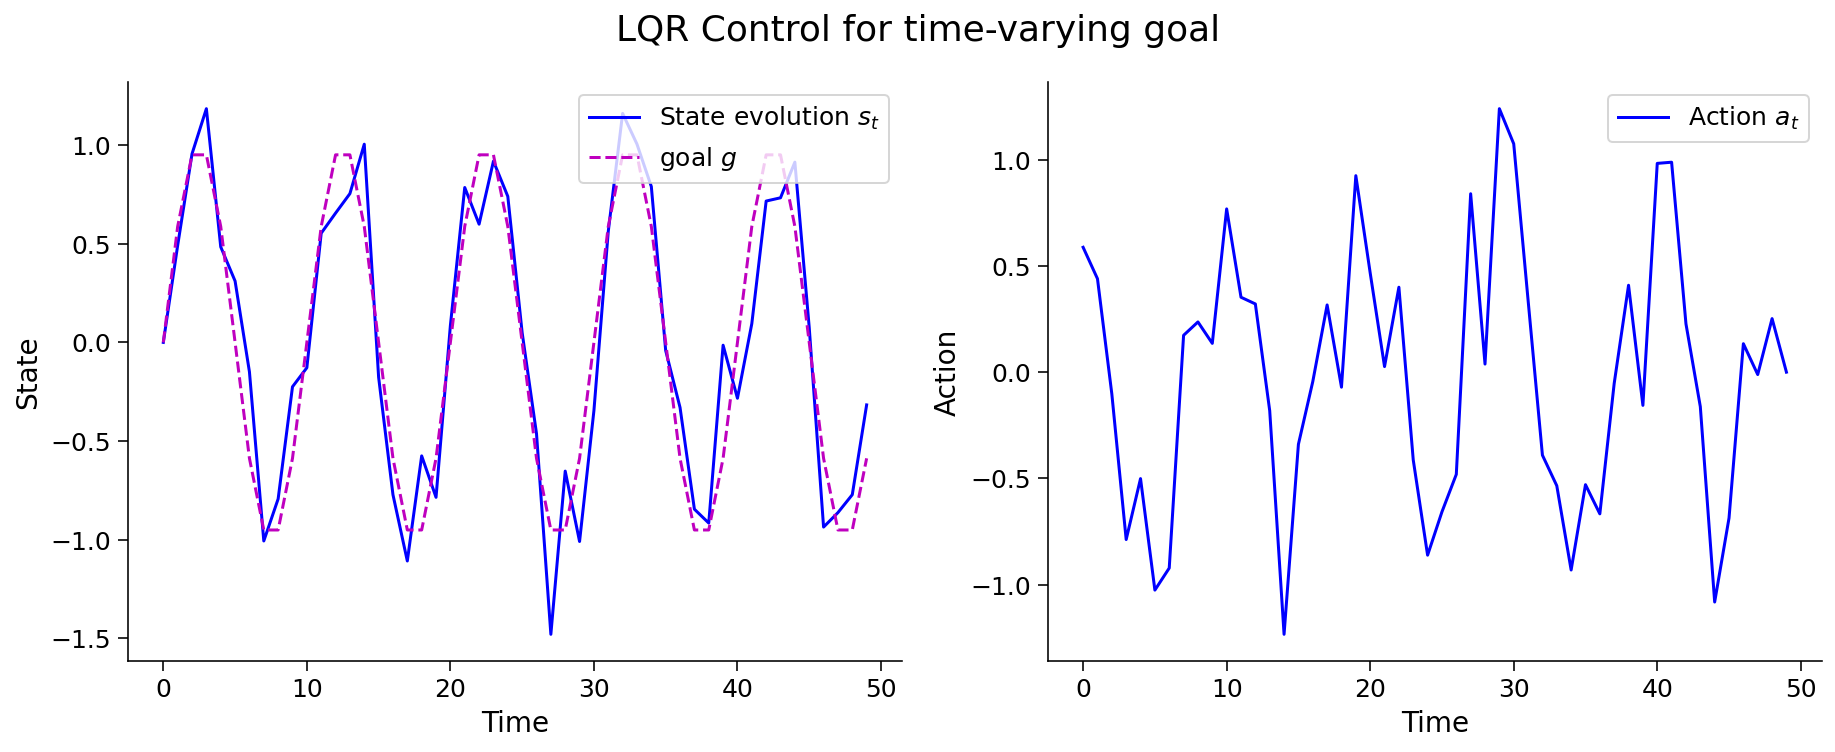
\includegraphics[scale=0.2]{Figures/OC/OC_Figure11.png}
\end{center}

\end{subbox}
\end{textbox}
%%%%%%%%%%%%%%%%%%%%%%%%% 
%%%%%%%%%%%%%%%%%%%%%%%%%
\begin{textbox}{\href{https://compneuro.neuromatch.io/tutorials/W3D3_OptimalControl/student/W3D3_Tutorial2.html}{Optimal Control for Continuous State}}
\begin{subbox}{subbox}{  Control of an partially observed state using a Linear Quadratic Gaussian (LQG) controller}
\scriptsize

In practice, the controller does not have full access to the state. For example, your jet pack in space may be controlled by Mission Control back on earth!  In this case, noisy measurements $m_t$ of the state $s_t$ are taken via radar, and the controller needs to (1) estimate the true state, and (2) design an action based on this estimate. \\

Fortunately, the separation principle tells us that it is optimal to do (1) and (2) separately. This makes our problem much easier, since we already know how to do each step.  \\

1) \textit{State Estimation}\\  
Can we recover the state from the measurement? 
yesterday you learned that the states $\hat{s}_t$ can be estimated from the measurements $m_t$ using the \textbf{Kalman filter}. \\

2) \textit{Design Action}  \\
We learned about the LQR controller which designs an action based on the state. The separation principle tells us that it is sufficient to replace the use of the state in LQR with the \textit{estimated} state, i.e.,

\begin{equation}
a_t = L_t \hat s_t
\end{equation}

The state dynamics will then be:

\begin{equation}
s_{t+1} = D s_t + B a_t + w_t
\end{equation}

where $w_t$ is the process noise (proc_noise), and the observation / measurement is:

\begin{equation}
m_t = C s_t + v_t
\end{equation}

with $C$ is the observation matrix and $v_t$ is the measurement noise (meas_noise).

The combination of (1) state estimation and (2) action design using LQR is known as a \textbf{linear quadratic gaussian (LQG)}. Yesterday, you completed the code for the Kalman filter. Based on that, you will code up the LQG controller. 
For these exercises, we will return to using the goal $g=0$, as in Section 2.

\end{subbox}

\end{textbox}
%%%%%%%%%%%%%%%%%%%%%%%%% 
%%%%%%%%%%%%%%%%%%%%%%%%%
\begin{textbox}{\href{https://compneuro.neuromatch.io/tutorials/W3D3_OptimalControl/student/W3D3_Tutorial2.html}{Optimal Control for Continuous State}}
\begin{subbox}{subbox}{  The Kalman filter in conjunction with a linear closed-loop controller (LQG Control)}
\scriptsize


\begin{center}
    
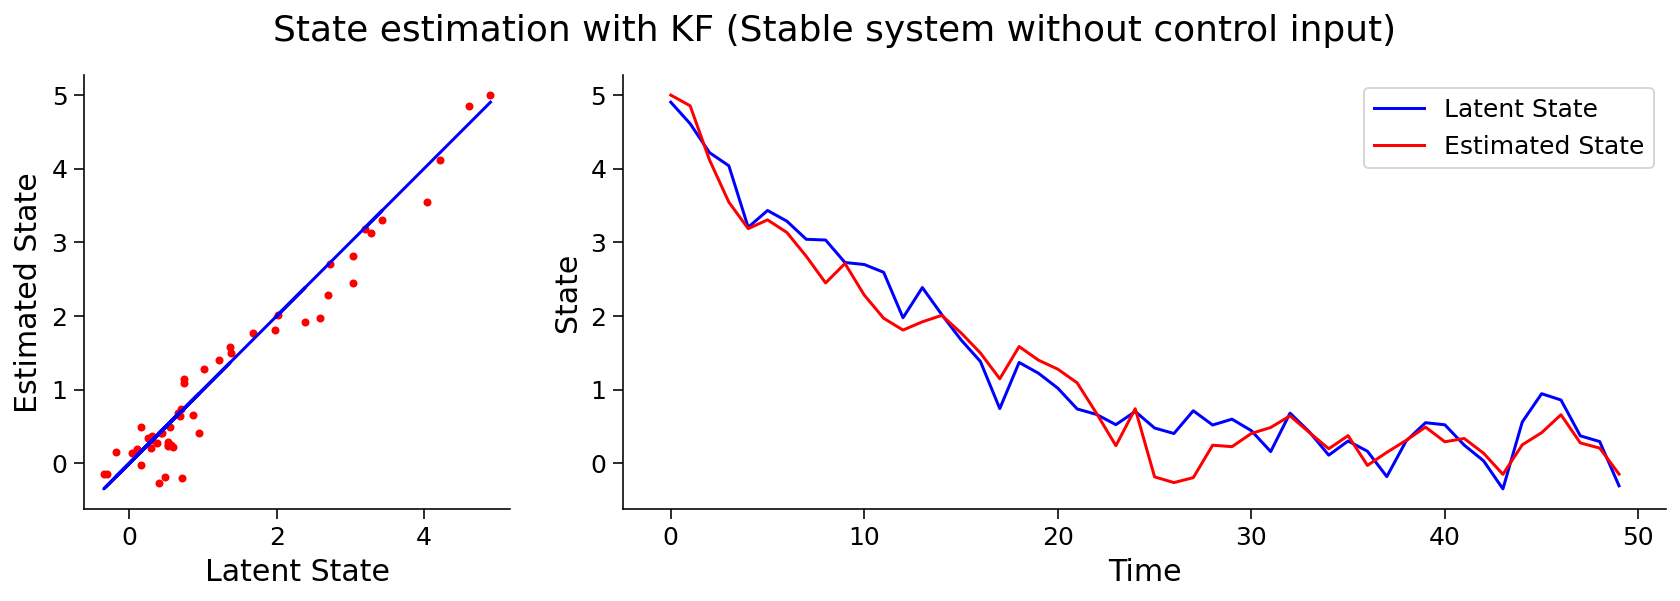
\includegraphics[scale=0.2]{Figures/OC/OC_Figure12.png}
\end{center}


\end{subbox}

\begin{subbox}{subbox}{  LQG controller output with varying control gains}
\scriptsize
Here the Kalman filter with closed-loop feedback with the controller. We will first use an arbitrary control gain and a fixed value for measurement noise. We will then use the control gain that we calculated for the LQR system given different values for $\rho$ (weight on the control effort).
\begin{enumerate}
    \item 
 Visualize the system dynamics $s_t$ in closed-loop control with an arbitrary constant control gain. Vary this control gain.

 \item  Play arround with the remaining sliders. What happens when the process noise is high (low)? How about the measurement noise?
\end{enumerate}

\begin{center}
    
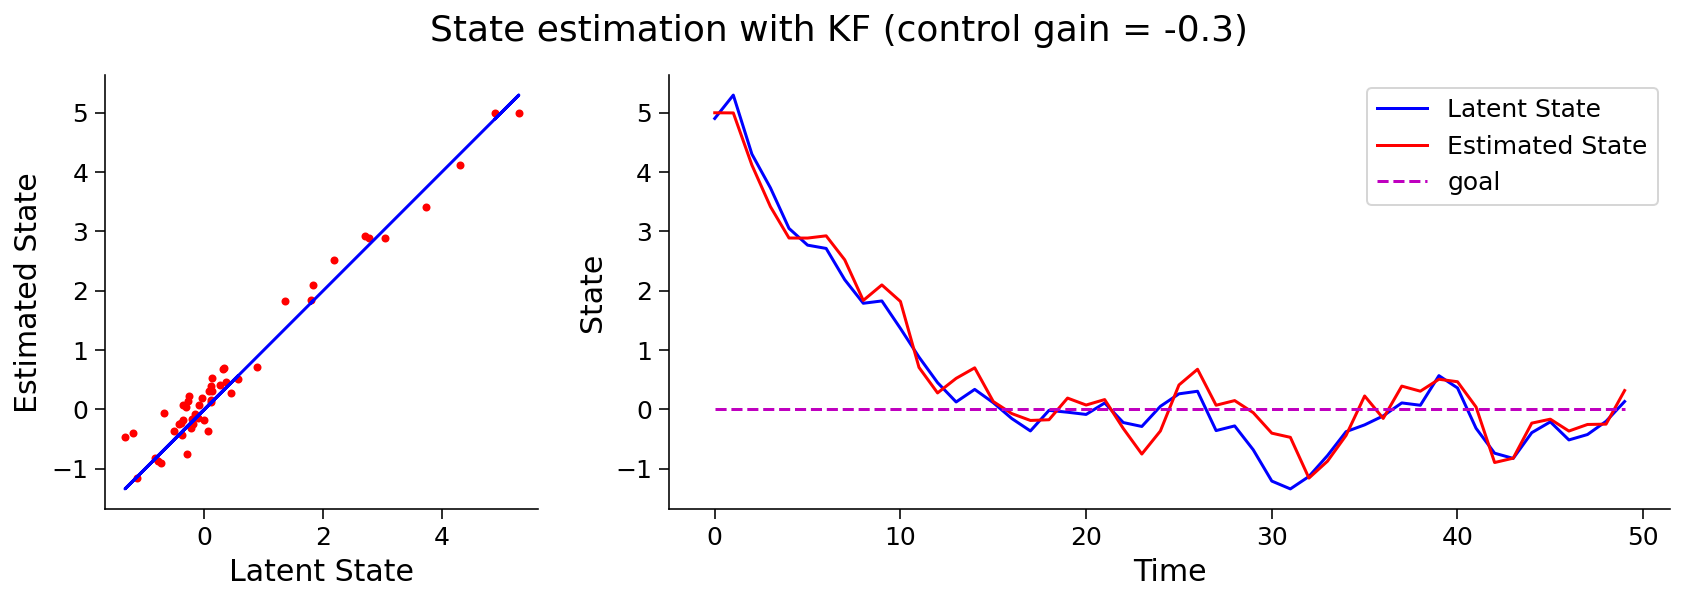
\includegraphics[scale=0.2]{Figures/OC/OC_Figure13.png}
\end{center}


\end{subbox}

\begin{subbox}{subbox}{LQG controller with varying weight on the control effort costs}
\scriptsize

Now let's see the performance of the LQG controller as the parameter $\rho$ changes. We will use an LQG controller gain, where the control gain is from a system with an infinite horizon; in this case, the optimal control gain turns out to be a constant.


\begin{center}
    
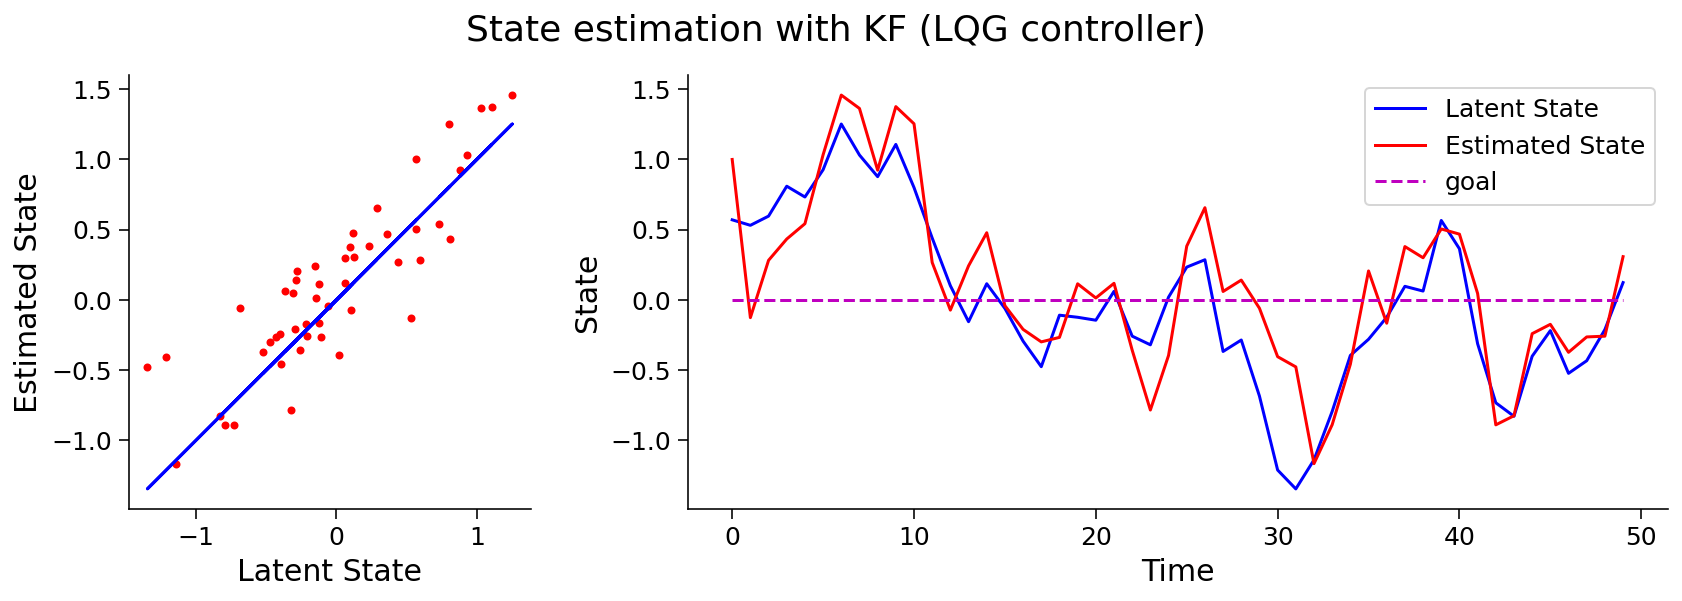
\includegraphics[scale=0.2]{Figures/OC/OC_Figure14.png}
\end{center}


\end{subbox}

\end{textbox}
%%%%%%%%%%%%%%%%%%%%%%%%% 
%%%%%%%%%%%%%%%%%%%%%%%%%
\begin{textbox}{\href{https://compneuro.neuromatch.io/tutorials/W3D3_OptimalControl/student/W3D3_Tutorial2.html}{Optimal Control for Continuous State}}
\begin{subbox}{subbox}{  How does the process noise and the measurement noise influence the controlled state and desired action?}
\scriptsize

Process noise $w_t$ and measurement noise $v_t$ have very different effects on the controlled state. 


\begin{center}
    
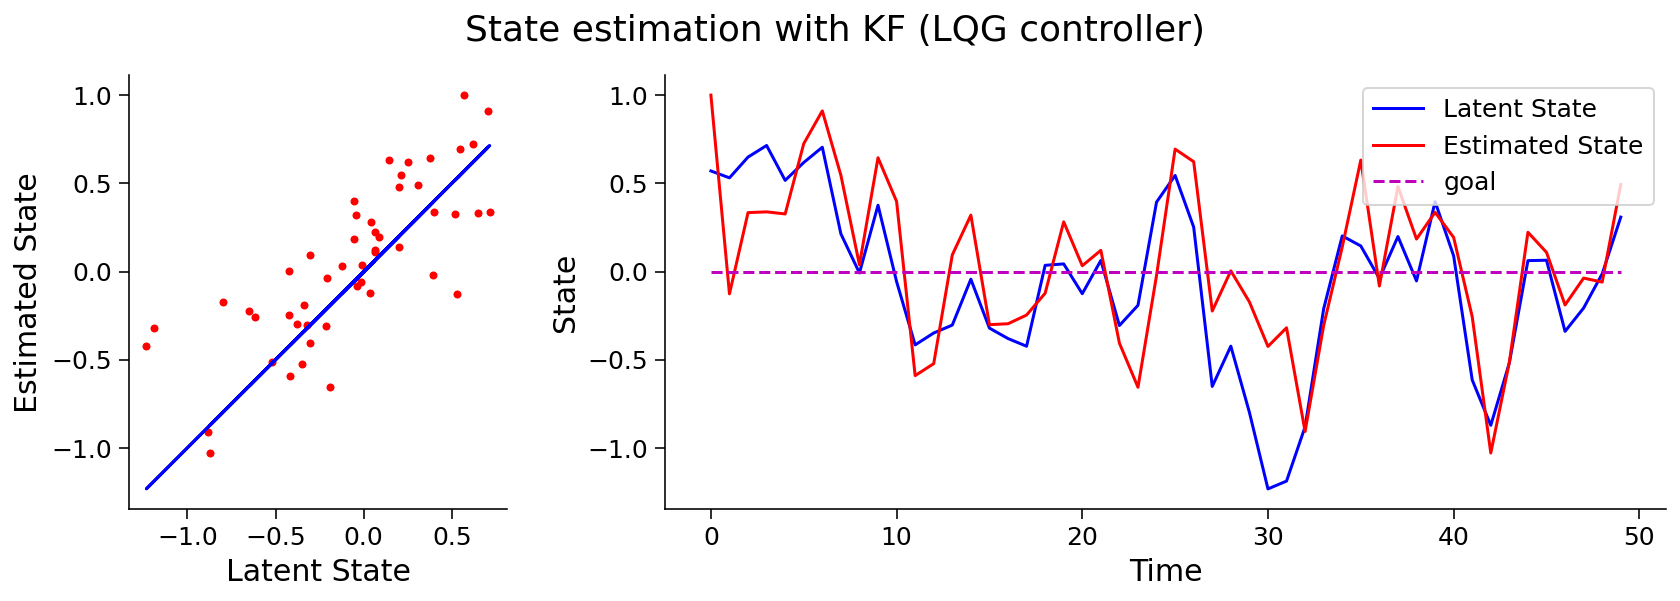
\includegraphics[scale=0.2]{Figures/OC/OC_Figure15.png}
\end{center}


\end{subbox}

\begin{subbox}{subbox}{  Noise effects on the LQG}
\scriptsize

Finally, we will quantify how the state cost and control costs change when we change the process and measurement noise levels. To do so, we will run many simulations, stepping through levels of process and measurement noise, tracking MSE and cost of control for each. 

Observe the effects of increasing the process and measurement noises in an unstable system. How do you interpret the results?

\begin{center}
    
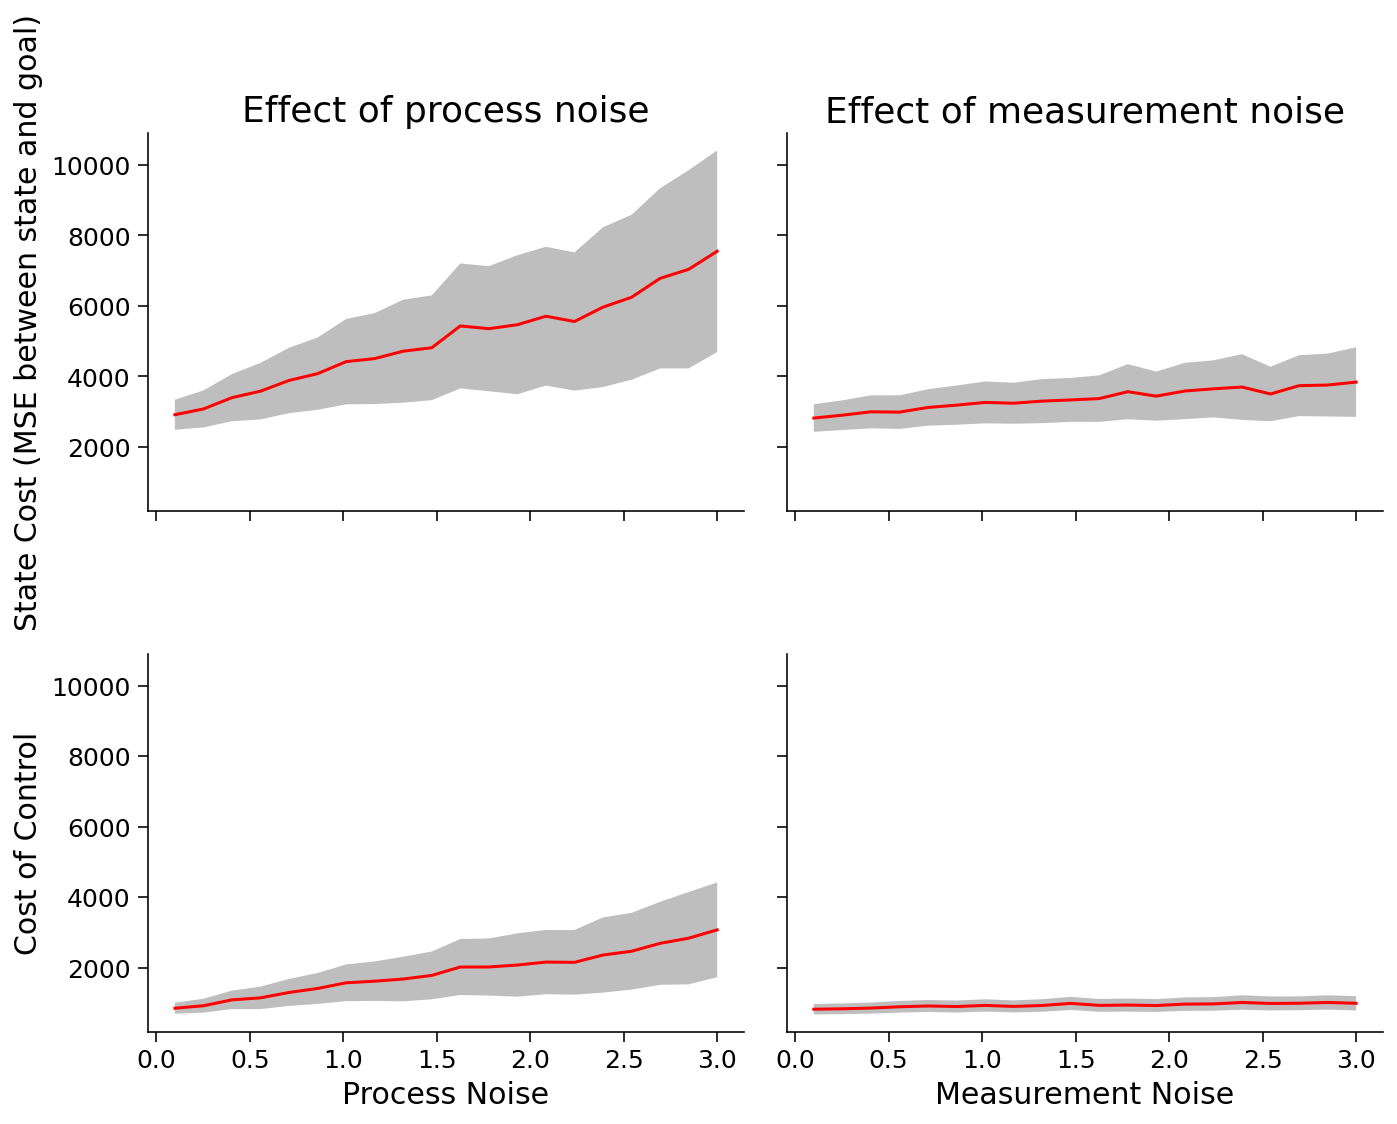
\includegraphics[scale=0.2]{Figures/OC/OC_Figure16.png}
\end{center}

While both sources of noise have an effect on the controlled state, the
process noise has a much larger effect. As the process noise w[t] increases,
state cost (MSE between state and goal) and  control cost increase drastically.
You can get an intuition as to why using the sliders in the demo above.  To make
matters worse, as the process noise gets larger, you will also need to put in
more effort to keep the system close to the goal.
The measurement noise v[t]  also has an effect on the accuracy of the
controlled state. As this noise increases, the MSE between the state and goal
increases. The cost of control in this case remains fairly constant with
increasing levels of measurement noise.

\end{subbox}
\end{textbox}
%%%%%%%%%%%%%%%%%%%%%%%%% 
%%%%%%%%%%%%%%%%%%%%%%%%%